\documentclass[10pt,a4paper, twoside]{article}

\usepackage[english]{babel} %English
\usepackage{graphicx}
\usepackage{textcomp}
\usepackage{amsfonts,amsmath,amssymb}
\usepackage[T1]{fontenc} 
\usepackage[utf8]{inputenc}
\usepackage{array}
\usepackage{tikz}
\usepackage{wrapfig}
\usepackage{lastpage}
\usepackage{fancyhdr}
\usepackage{color}
\usepackage{hyperref}
\usepackage{appendix}
\usepackage{url}

\usepackage{listings}
\lstset{language=Verilog,basicstyle=\tiny\ttfamily}

\pagestyle{fancy}

\definecolor{blue}{RGB}{0,78,138}
\definecolor{dkgreen}{rgb}{0,0.6,0}
\definecolor{gray}{rgb}{0.5,0.5,0.5}
\definecolor{mauve}{rgb}{0.58,0,0.82}

\lstset{
  language=tcl,						% the language of the code
  basicstyle=\small\ttfamily,		% the size of the fonts that are used for the code
  numbers=left,                   % where to put the line-numbers
  numberstyle=\tiny\color{gray},  % the style that is used for the line-numbers
  stepnumber=1,                   % the step between two line-numbers. If it's 1, each line 
                                  % will be numbered
  numbersep=5pt,                  % how far the line-numbers are from the code
  backgroundcolor=\color{white},      % choose the background color. You must add \usepackage{color}
  showspaces=false,               % show spaces adding particular underscores
  showstringspaces=false,         % underline spaces within strings
  showtabs=false,                 % show tabs within strings adding particular underscores
  frame=single,                   % adds a frame around the code
  rulecolor=\color{black},        % if not set, the frame-color may be changed on line-breaks within not-black text (e.g. commens (green here))
  tabsize=4,                      % sets default tabsize to 2 spaces
  captionpos=b,                   % sets the caption-position to bottom
  breaklines=true,                % sets automatic line breaking
  breakatwhitespace=false,        % sets if automatic breaks should only happen at whitespace
  title=\lstname,                 % show the filename of files included with \lstinputlisting;
                                  % also try caption instead of title
  keywordstyle=\color{dkgreen},   % keyword style
  commentstyle=\color{blue},      % comment style
  stringstyle=\color{mauve}\ttfamily,      % string literal style
  escapeinside={\%*}{*)},         % if you want to add a comment within your code
  morekeywords={*,...}            % if you want to add more keywords to the set
}

\lstdefinelanguage{SystemVerilog}{
  keywords={always_ff, always_comb, if, begin, end, else, case, endcase, typedef, const, logic, integer, assign, parameter, localparam, module, posedge, negedge, enum, input, output},
  keywordstyle=\color{blue}\bfseries,
  ndkeywords={class, export, boolean, throw, implements, import, this},
  ndkeywordstyle=\color{darkgray}\bfseries,
  identifierstyle=\color{black},
  sensitive=false,
  comment=[l]{//},
  morecomment=[s]{/*}{*/},
  commentstyle=\color{red}\ttfamily,
  stringstyle=\color{red}\ttfamily,
  %morestring=[b]',
  morestring=[b]"
}




\addtolength{\headheight}{48pt}
%top
%%\setlength{\voffset}{-1.0cm}
\setlength{\voffset}{-1.5cm}
%\setlength{\headsep}{1.7cm}
\setlength{\textwidth}{15cm}
\setlength{\headwidth}{15cm}
%\setlength{\footwidth}{15cm}
%\setlength{\marginparsep}{0.2cm}
%\setlength{\marginparwidth}{1.5cm}

%side
\setlength{\hoffset}{+0.44cm}
\setlength{\oddsidemargin}{+1.0cm}
\setlength{\evensidemargin}{-1.0cm}

%\fancyhead{}
%\fancyfoot{}

\fancyhead[LO, LE]{
\includegraphics[width=2.3cm]{figs/ies}}
\fancyhead[RO, RE]{
\includegraphics[width=5.0cm]{figs/athene}}
\fancyhead[CO, CE]{
\raisebox{0.78cm}{\parbox{10cm}{
\begin{flushleft}
\color{blue}
\hspace*{0.75cm}Prof. Dr.-Ing. Hofmann\\
\hspace*{0.75cm}Integrated Electronic Systems Lab\\
\hspace*{0.75cm}Merckstr. 25, D-64283 Darmstadt\\
\end{flushleft}}}
}
\fancyfoot[LE, LO]{
\color{blue}
%Dipl.-Ing. Boris Traskov\\
%\href{mailto:boris.traskov@ies.tu-darmstadt.de}{boris.traskov@ies.tu-darmstadt.de}
}

\fancyfoot[CE,CO] { }
\fancyfoot[RO,RE] {page \thepage\ of \pageref{LastPage}}
\renewcommand{\headrulewidth}{0.4pt}
\renewcommand{\footrulewidth}{0.4pt}

\title{HDL Lab Manual 2017}


\pagestyle{fancy}
\begin{document}
\thispagestyle{fancy}
\maketitle

\thispagestyle{fancy}
\tableofcontents
\thispagestyle{fancy}

\newpage
\thispagestyle{fancy}

% one page
\section{Introduction}
%TODO
% motivation / goals / work distribution 
\section{Primary Objectives}

\subsection{Processor Design in Verilog}
Design a processor that can execute \textit{Thumb} instructions
 for the instruction set given in the Thumb Quick Reference Card \cite{QRC}. Implement all instructions in the following sections: Move, Add, Subtract, Multiply, Compare, Logical, Shift/Rotate, Load, Store, Push, Pop, If-Then, Branch, Extend, Reverse, No Op. Do not implement Processor State Change and Hint. Refer to the ARM Architecture Manual \cite{ARMARM} for a detailed description of the instruction set. \\

The entire program code is stored in a 4Kx16 fully-buffered, single-port random access memory (RAM). 4Kx16 means that it has 4096 entries (depth) of 16 bit (width) each and it can store 8KB (B = byte, b = bit) in total. Fully-buffered means that its inputs as well as its outputs are registered. On a write, the memory contents update with the next rising edge of the clk input. On a read, the data is delayed by one cycle before appearing at the output.
Use the same clock signal for both cpu and memory. Only use active-high synchronous resets on all Flip-flops. Do not use Latches. Do not use tri-state logic.

\subsubsection*{Internal Structure}
An instruction set does not yet define the implementation of the cpu. It merely defines which registers exist, which instructions the cpu can process, what an instruction means etc. Therefore the architecture is up to you to decide.
Hint: Try to stick to the basic structure in the section ``Best Practices''.

\subsection{Register-Transfer-Level Simulation and Verification}
There are many ways to verify a design's correctness. In this lab you will create a \textit{directed test bench} and simulate it in Modelsim (a tutorial is provided in \cite{mentor}). This means you will define test cases in the form of C-programs as in appendix \ref{c:count32}. Using the provided makefile in appendix \ref{makefile} you can compile your test programs into ARM-assembler language files (.asm), executable and linkable files (.elf) and binary files (.bin).\\
Keep these programs simple as you will need to trace the program execution on your waveform viewer. When writing test programs also specify the correct expected results (golden model).\\
Once this is done you will simulate your DUT (device under test, i.e. cpu) with these test cases as memory content (stimulus) and compare the final memory content with the expected results.\\
\begin{itemize}
\item Review and understand the provided testbench and memory in the appendix. Use it as your starting point and adapt it where needed.
\item Write test programs (and document them) to ensure that all instructions work properly.
\item You are allowed to share test programs and verify your design with other groups' test programs. Give them credit in your report!
\item Include an active-high finish\_out signal in your design and assert it, when your program is done.
\end{itemize}

\subsection{Standard-Cell Synthesis}
\subsubsection{Synthesis using TSMC 45nm Standard Cells}
During the design process you will frequently synthesize your design with Design Compiler. You will use standard cell libraries from TSMC 45nm technology. The tool will tell you how fast your circuit will be.\\
As a rule of thumb: Code that you write should be synthesized by the end of the day. (In the beginning try lots of small iterations. Later - when you know what you are doing - try longer iterations.)\\
Take a look at your implementation reports and understand key metrics:
\begin{itemize}
\item frequency
\item (critical path delay)
\item area
\item power
\end{itemize} Be able to explain these metrics. When optimizing your design, observe how key metrics correlate with each other.

\subsubsection{Gate-Level Simulation and Verification}
Synthesis transforms your register-transfer-level design (RTL) into a gate-level design (GL). This is a net list of standard cells. Simulating on this net list allows you to verify functionality at gate level. A tutorial is provided in appendix \ref{tut:gls}.\\
Once at the end of each week make sure, that your example programs simulate correctly as in your RTL simulations. For fully-synchronous single-clocked designs you should not expect any surprises here. In asynchronous or multi-clock designs you'll be able to find bugs on gate-level that did not occur at register-transfer-level.\\
When you simulate on GL look at the waveforms and observe the switching activity. Review the terms slack, critical path and setup time.





\newpage
\section{Secondary Objectives}
When you are confident to have a functionally correct and synthesizable design you are ready to advance to the secondary objectives. The main task in this section is to 
\textbf{optimize for execution time} by using the techniques described in the following subsections. The basic optimization cycle starts with an evaluation of your current design. Once you have found and understood a performance bottleneck you will think of ways to push the limits, implement additional circuitry and start over.  Document your key figures and reasoning in each design refinement step. In most cases there is no optimal solution (or it's hard to tell before you try it out).
Before you start coding any of the following extensions:
\begin{itemize}
\item Write a program, to demonstrate the extension's effectiveness. Calculate the speed increase. Note that sometimes it suffices to recompile an existing program with different compiler optimizations.
\item Think of how you want to integrate it in your processor. Is it an additional pipeline stage? Is it a modification to one (or more) existing pipeline stage(s)?
\item Always KISS: ''Keep it Simple and Stupid!'' (If nothing else, remember this)
\end{itemize}
After (and while) designing an extension:
\begin{itemize}
\item Make sure that you do not break your other test programs.
\end{itemize}

\subsection{Instruction/Data Cache}
If memory bandwidth lags behind cpu performance:
\begin{itemize}
\item Build a configurable cache with parameters:
\begin{itemize}
\item	CACHE\_ON=[0 | 1]\\
		determines if a cache is instantiated (1) or not (0).
\item	CACHE\_SIZE= [2 | 4 | 8 | 16 | 32]\\
		determines the number of words in your cache.
\item	Additional parameters as needed (depending on policy).
\end{itemize} 
\item Cache policy and associativity is up to you. (KISS)
\end{itemize}

\subsection{Branch Prediction}		 
If a long pipeline causes long latency at branches:
\begin{itemize}
\item Build a branch prediction unit with parameters:
\begin{itemize}
\item	BP\_ON=[0 | 1]\\
		determines if a branch predictor is instantiated (1) or not (0).
\item	Additional parameters as needed (depending on policy).
\end{itemize} 
\item Algorithm is up to you. (KISS)
\end{itemize}

\subsection{Superscalar Execution}
If cpu performance lags behind memory bandwidth:
\begin{itemize}
\item Duplicate (triplicate, ...) the execution unit and add additional circuitry for decoding and distributing instructions and handling hazards.
\item Use parameters:
\begin{itemize}
\item	SS\_<UNIT>=[ (default: 1) | 2 | 3... ]\\
		indicating which unit is duplicated, triplicated...\\
		Replace <UNIT> with DEC, EX or other appropriate name
\item	Additional parameters as needed.
\end{itemize} 
\end{itemize}

\subsection{Balanced Pipeline}
If cpu performance lags behind memory bandwidth:
\begin{itemize}
	\item Split execute stage in two or more stages and add additional circuitry to handle hazards.
	\item If you have registered all your execute-stage outputs properly, this is an easy task. Look up the DesignCompiler command ``balance\_registers''.
\end{itemize}
\newpage

\section{Best Practices}



\subsection{Coding}
\begin{itemize}
	\item Draw your schematics/state machines on paper before coding!
	\begin{itemize}
		\item Do not try to save paper!
		\item Clearly mark combinational logic in one color and non-combinational in another. 
\item leave out clocks and resets from your drawing... too messy	
	\end{itemize}
	\item Make one separate file for each module. Recommended granularity: A stage is a module, e.g. "execute.v, decode.v, ..." This split is actually finer-grained than absolutely necessary, but gives a nice, clean design.\\
	\item Instantiate all synthesizable modules within "cpu.v". Then instantiate "cpu.v" in ''testbench.sv". This gives a nice, clean structure.
	\begin{center}
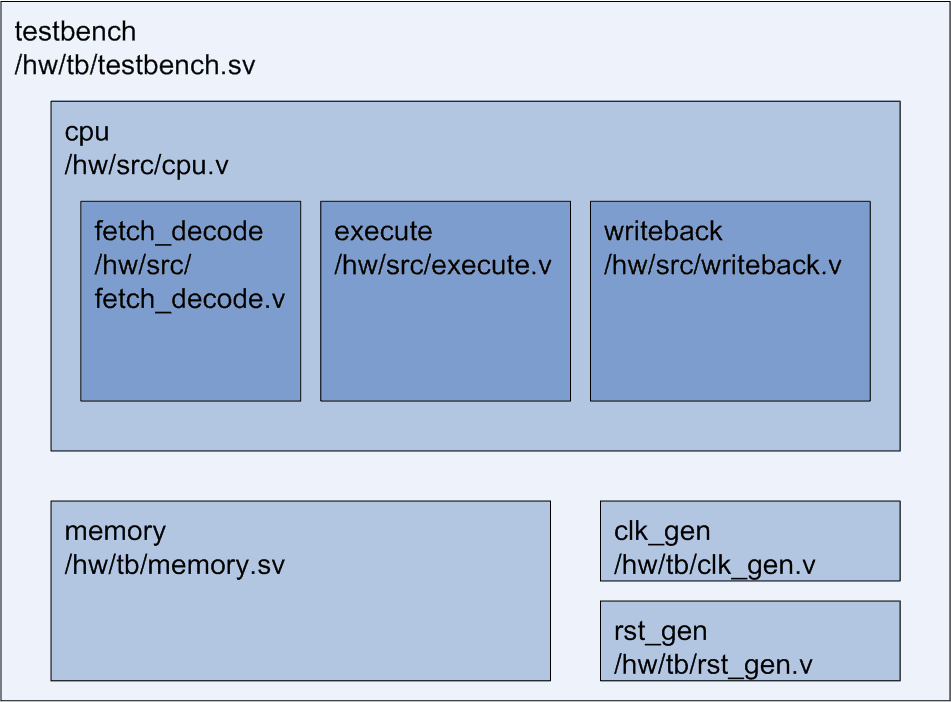
\includegraphics[width=6cm]{figs/block}
\end{center}
	\item Register all outputs of each stage, i.e. the output is driven by a register directly!
\begin{center}
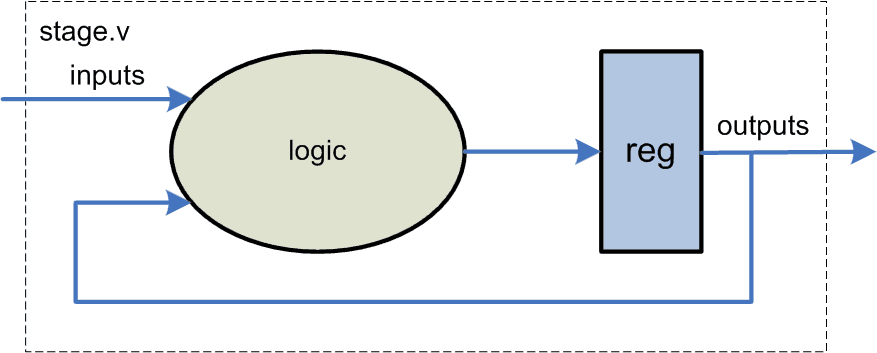
\includegraphics[width=6cm]{figs/stage}
\end{center}
This ''latched mealy'' machine is a very fast and safe technique to model pipelined data paths. (Mealy and Moore are taught in classes because they are difficult enough to confuse students. They are rarely used though, because of some poor properties: When connected together Mealy machines produce long combinational paths. Moore does not yield such long combinational paths but the basic drawback remains.)\\
%	Note 1: Inputs to a stage may be the outputs of any stage.\\
%	Note 2: Think twice whether you need a Mealy or Moore machine in your design.\\
%In short: One stage has inputs on the left, followed by combinational logic, followed by registers, followed by outputs.

	\item Decide upon a naming convention for signals, registers, modules, constants,...! Consistency helps when your code base grows larger and larger.
	\item Do not reinvent the wheel: Use the built-in operators ''+'' and ''-'' for addition and subtraction. The synthesis tool will infer the right architecture for you.
	\item No tri-state buses and no ''inout'' ports
	\item Port connections only by name, not by position
	\item Tasks/functions only if absolutely necessary
	\item Save your files often (at least once before lunch break and before leaving in the evening)! You can use a revision control system if you like.
	\item Comments, comments, comments
\end{itemize}


\subsection{Tools}
\begin{itemize}
	\item Do not run any tool in the same working directory in two shells at the same time. Instead have seperate working directories for each instance of the respective tool.
	\item Use the graphical user interface (GUI) to get familiar with the functionality. Later, you can observe the commands issued by the GUI to create your own scripts. The latter is preferred because it guarantees reproducibility. Also many useful commands/options are not available in the GUI.
\end{itemize}

\subsection{Group Work}
	\begin{itemize}
	\item Work together, discuss regularly and often.
	\item At least once a day (in the morning), discuss what each of you will do today.
	\item Work in pairs of 2 for a while, then come together to integrate your work. Explain what you did to the others. Make only small iterations!
	\item Make only small iterations! REALLY!
	\item Inform each other of your schedules/absences well in advance.
	\end{itemize}
\newpage
\section{Deliverables}
Make a folder tree as indicated below and place your files and your 1 page long short report named 
\begin{center}
\textbf{hdllab2017\_summary\_xx.pdf}
\end{center}
 in the corresponding sub-folder. Pack everything in a zip-file named 
\begin{center}\textbf{hdllab2017\_xx.zip}
\end{center}
 (xx is your group number) and email it to 
\begin{center}
\href{mailto:sarath.mohanan@ies.tu-darmstadt.de}{sarath.mohanan@ies.tu-darmstadt.de}\\
by\\
11.08.2017 (Friday) 23:59:59
\end{center}
In the short report indicate the major milestones achieved and status of your processor with respect to the test cases provided.

Make the detailed main report named 
\begin{center}
\textbf{hdllab2017\_report\_xx.pdf}
\end{center}
 and email it by 
\begin{center}

16.08.2017 (Wednesday) 23:59:59
\end{center}
\begin{enumerate}
	\item Folder structure
	\begin{itemize}
	    \item \textbf{/designs}		(gate-level netlists, .sdf timing anotation)
		\item \textbf{/documents}					(put your PDF report here)
		\item \textbf{/reports}						(synthesis reports: area, power, timing, resources, references)
		\item \textbf{/sources/rtl}					(RTL Verilog source code)
		\item \textbf{/source/scripts/simulation}			(simulation scripts)
		\item \textbf{/source/scripts/synthesis}			(synthesis scripts)
		\item \textbf{/source/sim}			       (Modlesim project directory)
		\item \textbf{/source/software}				(makefile, c-source files and binaries)
		\item \textbf{/source/syn}			       (Synthesis directory)
		\item \textbf{/source/testbench} 		   (testbench source code)
		\item \textbf{/stimulus}					(test program binaries)
		\end{itemize}
	
	\item Report (12 pages maximum, English)
		\begin{itemize}
		\item General outline
			\begin{itemize}		 
			\item Introduction / motivation / goals / work distribution (1 page)
			\item Implementation / technical work (10 pages)
				\begin{itemize}
				\item Design
					\begin{itemize}
					\item figure: block diagram of processor architecture
					\item Discussion of processor architecture
					\end{itemize}					
				\item RTL Verification
					\begin{itemize}
					\item figure: block diagram of testbench
					\item Discussion of testbench
					\end{itemize}		
				\item Synthesis
					\begin{itemize}
					\item figure: top level schematic
					\item Discussion of schematic
					\item figure: critical path schematic 
					\item Discussion of critical path 
					\item Discussion of resources and resource sharing
					\end{itemize}				
				\item GL Verification
				\item (other, e.g. comparison between different architectures... you can go crazy here)
				\end{itemize}		 
			\item Evaluation / conclusion (1 page)
				\begin{itemize}
				\item 
				\end{itemize}
			\item Appendix
				\begin{itemize}
				\item timing report
				\item resource report
				\item area report
				\item power report
				\end{itemize}
			\end{itemize}
		\item Hints
			\begin{itemize}
			\item There is no cookbook recipe (and only few mathematical formulas) for processor design, only good/bad experience. Therefore reports and articles in this domain need to focus on the reasoning, i.e. why a particular design was chosen. Sections on design iterations, evaluation strategies, comparisons between different options/configurations and so on are most interesting to read. 
			\item Use passive mode: ''The registers are comprised of d-flipflops'' instead of  ''we used d-flipflops for the registers''. In the work distribution (beginning) and conclusion (very end) sections you may use active mode, i.e. ''Sarath was responsible for the decode stage'' or ''the authors will continue verification after tape-out''.
			\item Express yourself clearly and in a concise form.					
			\item This is a good occasion to learn \LaTeX, because you will need it for your thesis. After the lab you are given sufficient days to write your report for exactly this reason.
			\end{itemize}
		\item Sad but true
		\begin{itemize}
			\item Plagiarism is embarrassing! Point out your own as well as others' original work. Cite when you use other people's results (even when paraphrasing). Ask if in doubt. All reports and source code at IES are checked with automated tools.
			\end{itemize}
	\end{itemize}
\end{enumerate}

\newpage
\section{Examination - HDL Lab}
The examination is mandatory, oral and takes place in groups of 4. It lasts roughly 30-45 minutes and the date is by agreement, preferably in the week after report submission. Use the following collection of questions for preparation. Read ``explain'' as ``tell a non-technical person how it works.'' If you are able to do so, then you can also explain it to your examinor.

\begin{enumerate}
		\item Know your group's design
			\begin{itemize}			
			\item Explain your general architecture. (What where your considerations when chosing this particular one?)
			\item Explain some line of your entire source code.
			\item Explain something that you have written (or omitted) in your report.
			\item Explain how an instruction passes through your design.
			\item Which is the most expensive operation in terms of time/area/power.
			\end{itemize}		
		\item Verilog
			\begin{itemize}			
			\item Write code for: DFF, sensitive to rising/falling edge with/without enable, with (a)synchronous reset
			\item Write code for: purely combinational barrel shifter that shifts din 0, 1, 2 or 3 bits right and drives dout with the result. Empty bits are filled with zeros. selection is based on signal ''shift'' (00, 01, 10, 11). din/dout have a width of 8.
			\item Write code for: some other simple logic/FSM ...	
			\end{itemize}	
		\item Digital Design
			\begin{itemize}
			\item Explain: Moore, Mealy, latched-Mealy
			\item Explain: 2's Complement, signed and unsigned representaion, carry and overflow
			\item Explain: combinational and non-combinational
			\item Explain: D-FF and Latch.
			\item Explain: setup time and hold time
			\item Explain: gtech library, synthetic library, Design Ware Building Blocks library
			\item Explain: critical path
			\item Explain: maximum frequency
			\item Explain: the power report
			\item Explain: the timing report
			\item Explain: the area report
			\item Explain: the reference report
			\end{itemize}
		\item Pipelining
			\begin{itemize}			
			\item What is the idea behind pipelining?
			\item Explain: hazard
			\item What types of hazards do you know? When do they occur? How can you resolve hazards?
			\item What is a balanced pipeline?
			\end{itemize}
		\item Other questions related to anything you did in the lab.
\end{enumerate}


%\newpage
\section{Technology Primers}


You have arrived at a point at which you have completed the HDL lab and go beyond coding Verilog. Feel free to go through these technology primers if you are interested. In each tutorial you will gain an impression of what is possible to do, and why it may be useful. It will be particularly useful to you if you plan to do a master thesis in digital design at IES or generally want to continue work in this domain.

\subsection{Introduction to Gate-Level Simulation}
\begin{itemize}
\item Simulate your cpu at gate-level and verify your synthesis procedure.
\end{itemize}

\subsection{Introduction to Power Simulation}
\begin{itemize}
\item Simulate your cpu at gate-level and verify your synthesis procedure.
\end{itemize}

\subsection{Introduction to Floorplanning}
\begin{itemize}
\item Simulate after place and route
\end{itemize}

\subsection{Introduction to Constrained Random Testing}
\begin{itemize}
\item Contrained random number generation
\item Property Specification language
\end{itemize}

\subsection{Introduction to SystemVerilog Direct-Programming-Interface}
If memory bandwidth lags behind cpu performance (or you are just interested).
\begin{itemize}
\item Understand and use a high-speed Memory Controller modelled in SystemC
\end{itemize}

\subsection{Introduction to SystemC}
If memory bandwidth lags behind cpu performance (or you are just interested).
\begin{itemize}
\item Understand and use a high-speed Memory Controller modelled in SystemC
\end{itemize}

\subsection{Introduction to Matlab/Modelsim Cosimulation}
If you want to evaluate whether your cpu can meet the demands for (place your application here) during the design process (or you are just interested).
\begin{itemize}
\item Model a simple IO-module and test it (IN and OUT instructions)
\item Set up a cosimulation environment with Matlab/Modelsim
\item Record an audio stream at 8 bit PCM and increase the volume by a factor of 2 with a) Matlab and b) your cpu. Make sure to saturate the signal correctly!
\end{itemize}

\subsection{Introduction to Intellectual Property Encryption}


\newpage
\begin{appendix}
\section{Timing report}
%TODO

\section{Resource report}
%TODO

\section{Area report}
%TODO

\section{Power report}
%TODO

\end{appendix}



\nocite{*}
\bibliography{bib}{}
\bibliographystyle{plain}



\end{document}
